% \documentclass[convert]{standalone}
\documentclass{standalone}
\usepackage[english]{babel}
% https://tex.stackexchange.com/questions/570303/use-blacktriangleright-as-itemize-label
\usepackage{amssymb} % for black triangleright

\renewcommand{\labelitemi}{$\textcolor{SwitchColor}{\bullet}$}
\renewcommand{\labelitemii}{$\textcolor{SwitchColor}{\blacktriangleright}$}

 \usepackage{csquotes}
\usepackage{xcolor}
% \usepackage{anyfontsize}
\usepackage{adjustbox}
% \usepackage[]{enumitem}
\usepackage{nicematrix}
\usepackage{tikz}
\usetikzlibrary{arrows.meta,positioning}
\usetikzlibrary{graphs}
\usetikzlibrary{patterns}
\usetikzlibrary{shadings}
\usetikzlibrary{mindmap, shadows, backgrounds} % , calc

\definecolor{PrimaryColor}{HTML}{5E3072}
\definecolor{PrimaryColorDimmed}{HTML}{a991cc}
\definecolor{SecondaryColor}{HTML}{EC6301}
\definecolor{SecondaryColorDimmed}{HTML}{ffbe99}
\colorlet{BoxColor}{gray!10!white}

\newlength{\leveldistance}
\setlength{\leveldistance}{18cm}

\begin{document}
  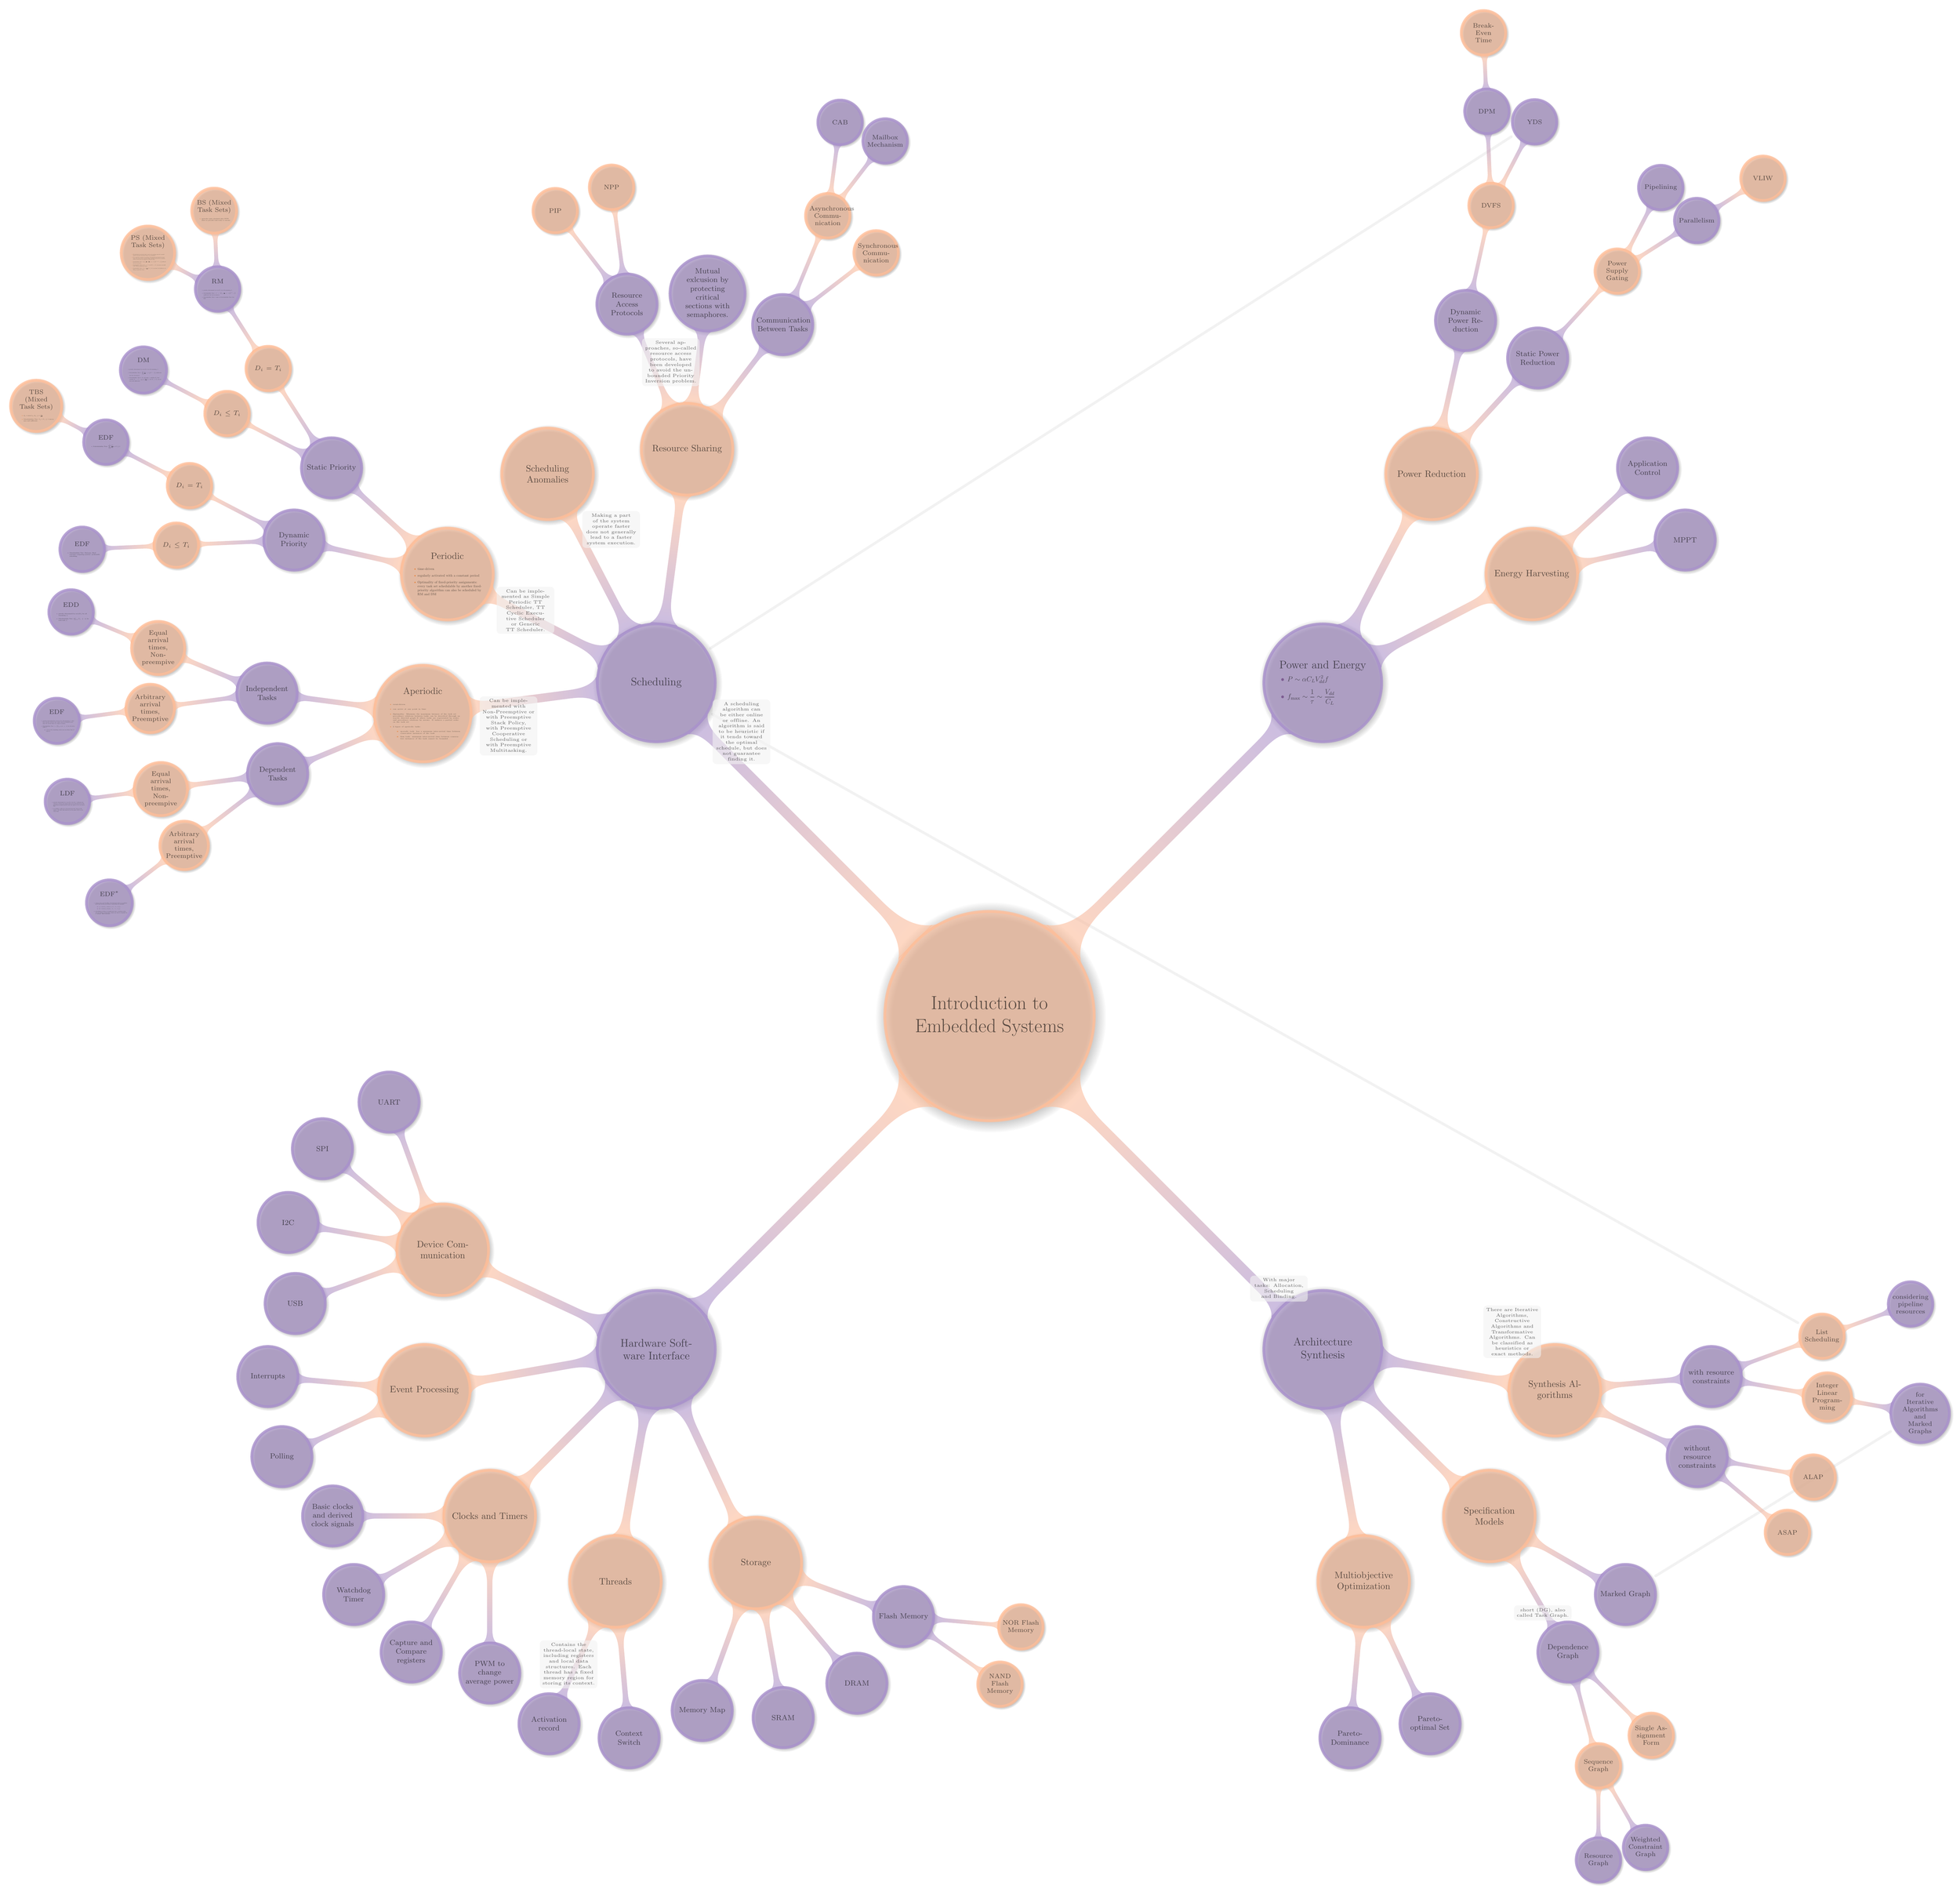
\begin{tikzpicture}[
      auto,
      huge mindmap,
      fill opacity=0.6,
      draw opacity=0.8,
      concept color = SecondaryColorDimmed,
      every annotation/.style={fill=BoxColor, draw=none, align=center, fill = BoxColor, text width = 2cm},
      grow cyclic,
      level 1/.append style = {
        concept color=PrimaryColorDimmed,
        level distance=\leveldistance,
        sibling angle=360/\the\tikznumberofchildren,
        % https://tex.stackexchange.com/questions/501240/trying-to-use-the-array-environment-inside-a-tikz-node-with-execute-at-begin-no
        execute at begin node=\definecolor{SwitchColor}{named}{PrimaryColor},
      },
      level 2/.append style = {
        concept color=SecondaryColorDimmed,
        level distance=\leveldistance / 2,
        sibling angle=35,
        execute at begin node=\definecolor{SwitchColor}{named}{SecondaryColor},
      },
      level 3/.append style = {
        concept color=PrimaryColorDimmed,
        level distance=\leveldistance / 3,
        execute at begin node=\definecolor{SwitchColor}{named}{PrimaryColor},
      },
      level 4/.append style = {
        concept color=SecondaryColorDimmed,
        level distance=\leveldistance / 4,
        execute at begin node=\definecolor{SwitchColor}{named}{SecondaryColor},
      },
      level 5/.append style = {
        concept color=PrimaryColorDimmed,
        level distance=\leveldistance / 5,
        execute at begin node=\definecolor{SwitchColor}{named}{PrimaryColor},
      },
      level 6/.append style = {
        concept color=SecondaryColorDimmed,
        level distance=\leveldistance / 6,
        execute at begin node=\definecolor{SwitchColor}{named}{SecondaryColor},
      },
      level 7/.append style = {
        concept color=PrimaryColorDimmed,
        level distance=\leveldistance / 7,
        execute at begin node=\definecolor{SwitchColor}{named}{PrimaryColor},
      },
      level 8/.append style = {
        concept color=SecondaryColorDimmed,
        level distance=\leveldistance / 8,
        execute at begin node=\definecolor{SwitchColor}{named}{SecondaryColor},
      },
      concept connection/.append style = {
        color = BoxColor,
      },
  ]
  % damit Annotationen nicht auch eine Drop Shadow erhalten
  \begin{scope}[
      every node/.style = {concept, circular drop shadow}, % draw=none
      every child/.style={concept},
    ]
  \node (ese) at (current page.center) {Introduction to Embedded Systems}
  child {
    node {Hardware Software Interface}
      child {
        node {Device Communication}
        child {
          node {UART}
        }
        child {
          node {SPI}
        }
        child {
          node {I2C}
        }
        child {
          node {USB}
        }
      }
      child {
        node {Event Processing}
          child {
            node {Interrupts}
          }
          child {
            node {Polling}
          }
      }
      child {
        node {Clocks and Timers}
        child {
          node {Basic clocks and derived clock signals}
        }
        child {
          node {Watchdog Timer}
        }
        child {
          node {Capture and Compare registers}
        }
        child {
          node {PWM to change average power}
        }
      }
      child {
        node {Threads}
        child {
          node (activationrecord) {Activation record}
        }
        child {
          node {Context Switch}
        }
      }
      child {
        node (storage) {Storage}
        child {
          node {Memory Map}
        }
        child {
          node {SRAM}
        }
        child {
          node {DRAM}
        }
        child {
          node {Flash Memory}
          child {
            node {NAND Flash Memory}
          }
          child {
            node {NOR Flash Memory}
          }
        }
      }
  }
  child {
    node (architecturesynthesis) {Architecture Synthesis}
      child {
        node {Multiobjective Optimization}
        child {
          node {Pareto-Dominance}
        }
        child {
          node {Pareto-optimal Set}
        }
      }
      child {
        node {Specification Models}
          child {
            node (dg) {Dependence Graph}
              child {
                node {Sequence Graph}
                  child {
                    node {Resource Graph}
                  }
                  child {
                    node {Weighted Constraint Graph}
                  }
              }
              child {
                node {Single Assignment Form}
              }
          }
          child {
            node (mg) {Marked Graph}
          }
      }
      child {
        node (synthesisalgorithms) {Synthesis Algorithms}
          child {
            node {without resource constraints}
            child {
              node {ASAP}
            }
            child {
              node {ALAP}
            }
          }
          child {
            node {with resource constraints}
              child {
                node {Integer Linear Programming}
                  child {
                    node (foriaandmg) {for Iterative Algorithms and Marked Graphs}
                  }
              }
              child {
                node (listscheduling) {List Scheduling}
                child {
                  node {considering pipeline resources}
                }
              }
          }
      }
  }
  child {
    node {Power and Energy
      \resizebox{\textwidth}{!}{
        \begin{minipage}[t]{6cm}
          \begin{itemize}
            \item $\begin{aligned}[t]P \sim \alpha C_L V_{d d}^2 f\end{aligned}$
            \item $\begin{aligned}[t]f_{\max } \sim \frac{1}{\tau} \sim \frac{V_{d d}}{C_L}\end{aligned}$
          \end{itemize}
        \end{minipage}
      }
    }
      child {
        node {Energy Harvesting}
          child {
            node {MPPT}
          }
          child {
            node {Application Control}
          }
      }
      child {
        node {Power Reduction}
          child {
            node {Static Power Reduction}
              child {
                node {Power Supply Gating}
                  child {
                    node {Parallelism}
                      child {
                        node {VLIW}
                      }
                  }
                  child {
                    node {Pipelining}
                  }
              }
          }
          child {
            node {Dynamic Power Reduction}
              child {
                node {DVFS}
                  child {
                    node (yds) {YDS}
                  }
                  child {
                    node {DPM}
                      child {
                        node {Break-Even Time}
                      }
                  }
                }
          }
        }
  }
  child {
    node (scheduling) {Scheduling}
      child {
        node (resourcesharing) {Resource Sharing}
          child {
            node {Communication Between Tasks}
              child {
                node {Synchronous Communication}
              }
              child {
                node {Asynchronous Communication}
                  child {
                    node {Mailbox Mechanism}
                  }
                  child {
                    node {CAB}
                  }
              }
          }
          child {
            node {Mutual exlcusion by protecting critical sections with semaphores.}
          }
          child {
            node (resourcesharingprotocols) {Resource Access Protocols}
              child {
                node {NPP}
              }
              child {
                node {PIP}
              }
          }
      }
      child {
        node (schedulinganomalies) {Scheduling Anomalies}
      }
      child {
        node (periodic) {Periodic
          \resizebox{\textwidth}{!}{
            \begin{minipage}[t]{8cm}
              \begin{itemize}
                \item time-driven
                \item regularly activated with a constant period
                \item Optimality of fixed-priority assignments: every task set schedulable by another fixed-priority algorithm can also be scheduled by RM and DM
              \end{itemize}
            \end{minipage}
          }
        }
        child {
          node {Static Priority}
          child {
            node {$D_i = T_i$}
            child [sibling angle=60] {
              node {RM
                \resizebox{\textwidth}{!}{
                  \begin{minipage}[t]{8cm}
                    \begin{itemize}
                      \item priority determined by $min(T_i)$ for all remaining $J_i$
                      \item Schedulability Test 1: $U=\sum_{i=1}^n \frac{C_i}{T_i} \leq n\left(2^{1 / n}-1\right)$ (sufficient but not necessary)
                      \item Schedulability Test 2: same as Schedulability Test 2 for DM
                    \end{itemize}
                  \end{minipage}
                }
              }
                child {
                  node {BS (Mixed Task Sets)
                    \resizebox{\textwidth}{!}{
                      \begin{minipage}[t]{6cm}
                        \begin{itemize}
                           \item aperiodic tasks scheduled after FCFS when no periodic task ready to execute
                        \end{itemize}
                      \end{minipage}
                    }
                  }
                }
                child {
                  node {PS (Mixed Task Sets)
                    \resizebox{\textwidth}{!}{
                      \begin{minipage}[t]{10cm}
                        \begin{itemize}
                          \item PS scheduled as periodic task, it serves any pending aperiodic requests until its capacity (execution time) Cs is exhausted
                          \item If no aperiodic requests are pending, PS suspends itself until the beginning of its next period, and the budget originally allocated for aperiodic service is freed up and assigned to periodic tasks
                          \item Schedulability Test 1: $\sum_{i=1}^n \frac{C_i}{T_i}+\frac{C_s}{T_s}\leq(n+1)\left[2^{1 /(n+1)}-1\right]$ (sufficient but not necessary)
                          \item Schedulability Test 2: If $C_a\le C_s$ and $2T_s\le D_a$ (necessary and sufficient, fitting computation time)
                          \item Schedulability Test 3: $T_S+\left\lceil \frac{C_a}{C_s}\right\rceil T_s \leq D_a$ (necessary and sufficient, not fitting computation time)
                        \end{itemize}
                      \end{minipage}
                    }
                  }
                }
            }
          }
          child {
            node {$D_i\le T_i$}
            child {
              node {DM
                \resizebox{\textwidth}{!}{
                  \begin{minipage}[t]{8cm}
                    \begin{itemize}
                      \item priority determined by $min(D_i)$ for all remaining $J_i$
                      \item Schedulability Test 1: $\displaystyle\sum_{i=1}^n \frac{C_i}{D_i} \leq n\left(2^{1 / n}-1\right)$ (sufficient but not necessary)
                      \item Schedulability Test 2: for all tasks $\tau_i$ smallest $R_i$ that satisfies $R_i=C_i+\sum_{j=1}^{i-1}\left\lceil\frac{R_i}{T_j}\right\rceil C_j$ and $R_i \le D_i$ (necessary and sufficient)
                    \end{itemize}
                  \end{minipage}
                }
              }
            }
          }
        }
        child {
          node {Dynamic Priority}
          child {
            node {$D_i = T_i$}
            child {
              node {EDF
                \resizebox{\textwidth}{!}{
                  \begin{minipage}[t]{6cm}
                    \begin{itemize}
                      \item Schedulability Test: $\displaystyle\sum_{i=1}^n \frac{C_i}{T_i}=U \leq 1$
                    \end{itemize}
                  \end{minipage}
                }
              }
              child {
                node {TBS (Mixed Task Sets)
                  \resizebox{\textwidth}{!}{
                    \begin{minipage}[t]{6cm}
                      \begin{itemize}
                        \item $d_k=\max \left(r_k, d_{k-1}\right)+\frac{C_k}{U_s}$
                        \item Schedulability Test: $U_p + U_s \le 1$ (necessary and sufficient)
                      \end{itemize}
                    \end{minipage}
                  }
                }
              }
            }
          }
          child {
            node {$D_i\le T_i$}
            child {
              node {EDF
                \resizebox{\textwidth}{!}{
                  \begin{minipage}[t]{6cm}
                    \begin{itemize}
                      \item Schedulability Test: Buttazzo, Hard real-time computing systems: predictable scheduling
                    \end{itemize}
                  \end{minipage}
                }
              }
            }
          }
        }
      }
      child {
        node (aperiodic) {Aperiodic
          \resizebox{\textwidth}{!}{
            \begin{minipage}[t]{8cm}
              \tiny
              \begin{itemize}
                \item event-driven
                \item can arrive at any point in time
                \item Optimality: Minimize the maximum lateness of the task set precedence relations between tasks can be described through an acyclic directed graph G where tasks are represented by nodes and precedence relations by arrows. G induces a partial order on the task set
                \item 2 types of aperiodic tasks:
                \begin{itemize}
                  \tiny
                  \item sporadic task: has a minimum inter-arrival time between consecutive instances of the task
                  \item firm task: minimum inter-arrival time between consecutive instances of the task cannot be bounded
                \end{itemize}
              \end{itemize}
            \end{minipage}
          }
        }
        child {
          node {Independent Tasks}
          child {
            node {Equal arrival times, Non-preempive}
            child {
              node {EDD
                \resizebox{\textwidth}{!}{
                  \begin{minipage}[t]{6cm}
                    \begin{itemize}
                      \item priority determined by $min(D_i)$ for all remaining $J_i$
                      \item Schedulability Test: $\sum_{k=1}^i C_k \leq d_i$ for each task $J_i$
                    \end{itemize}
                  \end{minipage}
                }
              }
            }
          }
          child {
            node (preemptive1) {Arbitrary arrival times, Preemptive}
              child {
                node {EDF
                  \resizebox{\textwidth}{!}{
                    \begin{minipage}[t]{8cm}
                      \begin{itemize}
                        \item priority determined by $min(d_i)$ for all remaining $J_i$ that have already arrived (are ready) and not finished every time the arrival time of a task is reached
                        \item Schedulability Test: $t+\sum_{k=1}^i c_k(t) \leq d_i$ for all active tasks $J_i$
                          \begin{itemize}
                            \item $c_k(t)$ is the remaining worst-case execution time of task $J_k$
                          \end{itemize}
                      \end{itemize}
                    \end{minipage}
                  }
                }
              }
          }
        }
        child {
          node {Dependent Tasks}
          child {
            node {Equal arrival times, Non-preempive}
            child {
              node {LDF
                \resizebox{\textwidth}{!}{
                  \begin{minipage}[t]{8cm}
                    \begin{itemize}
                      \item priority determined by $max(D_i)$ for all $J_i$ without successors or whose successors have been all selected in the precedence graph inserted into the queue to be executed last
                      \item at runtime, tasks are extracted from the head of the queue: the first task inserted in the queue will be executed last
                    \end{itemize}
                  \end{minipage}
                }
              }
            }
          }
          child {
            node (preemptive2) {Arbitrary arrival times, Preemptive}
            child {
              node {EDF$^*$
                \resizebox{\textwidth}{!}{
                  \begin{minipage}[t]{8cm}
                    \begin{itemize}
                      \item release time and deadline of individual tasks are modified such that all the precedence constraints are satisfied
                        \begin{itemize}
                          \item $r_j^* = max(r_j, max(r_i^* + C_i : J_i \rightarrow J_j))$
                          \item $d_i^* = min(d_i, min(d_j^* - C_j : J_i \rightarrow J_j))$
                        \end{itemize}
                      \item scheduling problem is transformed into a problem without precedence constraints, which can then be handled by a ”normal” EDF scheduler
                    \end{itemize}
                  \end{minipage}
                }
              }
            }
          }
        }
      }
  };
  \end{scope}
  % ┌───────────────────┐
  % │ Verbindungslinien │
  % └───────────────────┘
  \begin{pgfonlayer}{background}
  \draw [concept connection]
      (yds) edge (scheduling)
      (listscheduling) edge (scheduling)
      (foriaandmg) edge (mg);
  \end{pgfonlayer}
  % ┌──────────────┐
  % │ Annotationen │
  % └──────────────┘
  % https://tex.stackexchange.com/questions/302976/node-positioning-middle-point-mind-map-connection-bar
  \path (activationrecord) -- node[annotation, above, align=center, pos=0.01] {Contains the thread-local state, including registers and local data structures. Each thread has a fixed memory region for storing its context.} (ese);
  \path (periodic) -- node[annotation, above, align=center, pos=0.1] {Can be implemented as Simple Periodic TT Scheduler, TT Cyclic Executive Scheduler or Generic TT Scheduler.} (ese);
  \path (aperiodic) -- node[annotation, above, align=center, pos=0.1] {Can be implemented with Non-Preemptive or with Preemptive Stack Policy, with Preemptive Cooperative Scheduling or with Preemptive Multitasking.} (ese);
  \path (scheduling) -- node[annotation, above, align=center, pos=0.2] {A scheduling algorithm can be either online or offline. An algorithm is said to be heuristic if it tends toward the optimal schedule, but does not guarantee finding it.} (ese);
  \path (resourcesharingprotocols) -- node[annotation, above, align=center, pos=0.1] {Several approaches, so-called resource access protocols, have been developed to avoid the unbounded Priority Inversion problem.} (ese);
  \path (schedulinganomalies) -- node[annotation, above, align=center, pos=0.1] {Making a part of the system operate faster does not generally lead to a faster system execution.} (ese);
  \path (dg) -- node[annotation, above, align=center, pos=0.01] {short (DG), also called Task Graph.} (ese);
  \path (architecturesynthesis) -- node[annotation, above, align=center, pos=0.01] {With major tasks: Allocation, Scheduling and Binding.} (ese);
  \path (synthesisalgorithms) -- node[annotation, above, align=center, pos=0.01] {There are Iterative Algorithms, Constructive Algorithms and Transformative Algorithms. Can be classified as heuristics or exact methods.} (ese);
  \end{tikzpicture}
\end{document}
